\documentclass[main.tex]{subfiles}

\begin{document}
In this Chapter we will derive the \emph{Linear Power Flow} (LPF) transformation: a linear map from the vector of power injections at the buses to the vector of currents flowing through the lines of the network.

It is a \emph{right inverse} of $\FRT$, which means that applying $\LPF$ to a power injection gives a flow that would induce that injection. There are many possible candidates for a right inverse. One way to construct one is to fix a minimum spanning tree. When we set line currents outside of the tree to zero, all line currents inside the tree are uniquely determined.

Yet, only one right inverse is \emph{physically correct}: the $\LPF$. This function can be derived explicitly by constructing an electric circuit that represents the whole transmission network and everything connected to it, and applying Ohm's Law and Kirchoff's Laws to relate line currents to power injections. We linearise the resulting \emph{node flow equations} to find the LPF matrix (page \pageref{eq:LPF}).

Using this linear map, we can transform the normal distribution of stochastic injections to a Gaussian distribution of line flows. Using the results of Chapter \ref{chap:probability}, we can estimate the overload probability of each line, resulting in a ranking of most vulnerable lines. Additionally, for each such line, we compute the most probable injection to cause the failure, and simulate the subsequent \emph{cascading failures}.

\section{The model}
The $\LPF$ is essentially the \emph{high-level model} used in the final chapters of this thesis (\ie the transmission network is modelled as a linear transformation). In this chapter, we derive a closed-form expression for the $\LPF$ from a lower-level, \emph{electrical} model.

\subsection{Electrical model}
We make a distinction between the \emph{structure} and the \emph{state} of the network. The structure is a directed graph, where each line is given an \emph{admittance}. The state collects the (real and reactive) power injected at each bus, the (complex) voltage of each bus, and the (complex) current flowing through each line.

The use of complex-valued voltage and current (and therefore power) is essential when analysing AC circuits, even though we are only interested in \emph{real} power. For example, we will find that the amount of real power transmitted over a line is approximately inversely proportional to the inductance of the line (the \emph{imaginary} equivalent of resistance), and approximately proportional to the difference in phase angles at its ends (the \emph{complex argument} of voltage).
% Feynman: What I cannot create, I do not understand.
%This approach attempts to combine mathematical and physical theory, while maintaining a clear distinction between the two.

\subsection{Time invariance}
The grid structure remains unchanged during normal operation, while the grid state is continually changing over time. For example, an important aspect of grid operation is \define{load profiling}: examining and predicting the total load connected to a node, as a function of time. As a result of changing loads, the flow of power in a grid is constantly changing.

One example of a change in grid structure is a \emph{line failure}, which can be modelled as the removal of an edge from the graph. In some cases, the removal of an edge from the graph result in an unconnected graph (\ie there exist two nodes with no sequence of lines connecting them). This scenario is called \emph{power islanding}\index{power island}.
Most transmission networks are designed in such a way that no single (or double) line failure can cause power islanding or a blackout, by increasing the \emph{edge-connectivity} of the graph.

In the case of a \emph{line overload}, however, a line failure is caused by an exceptionally high power flow, as a result of high supply or demand.\footnote{These high power injections are not necessarily located at the two endpoints of an overloaded line; it could also be a grid-wide pattern of power injections, all adding up to a high power flow on that line. We will study the \emph{most likely power injection} in Chapter \ref{mostlikelypowerinjection}.}
The failure of an overloaded line will cause a redistribution of power flow, since the power flowing through the failed line now needs to 'find another path' between the nodes. In a highly stressed network, this redistribution can cause a second failure, which can then cause a third failure, and so on, eventually causing a blackout. We will study these \define{cascading failures} in Section \ref{sec:cascades}. \todo{We \emph{model} the line protection mechanism as deterministic: overload causes instantanious failure.}

\section{Grid structure}
A transmission grid is modelled as a directed graph $(\mathcal{N},\mathcal{L})$.\todo{Require the graph to be connected? How about power islands?} As vertices we take the \emph{nodes} of the network, which are those points where transmission lines connect to a generator, load, or to each other. Nodes are electrically distinct, in the sense that there is some non-zero impedance between them, allowing them to sustain a potential difference. In a network of $n$ nodes, they are represented by the natural numbers $1,\dots,n$, \ie $\mathcal{N}=\range{n}$.

A pair of two distinct nodes $(i,j)$ is contained in our set of lines $\mathcal{L}$ if there is a transmission line connecting the nodes. The choice of line orientation can be arbitrary, but we fix the orientation to $i<j$, \ie $(j,i) \notin \mathcal{L}$. This transmission line has non-zero impedance. (Otherwise $i$ and $j$ would be the same node.) In a network of $m$ lines, lines are labelled $\mathcal{L}_1, \dots, \mathcal{L}_m$. 

In literature on the subject, \todo{and in this thesis, oopsie} buses\footnote{`bus' is short for `busbar': the latin `omnibus' in conjunction with `bar': some high-voltage cables are connected by welding them to a heavy metal bar.} are also called \emph{vertices} or \emph{nodes}, and lines can be called \emph{edges}, \emph{wires}, \emph{cables} or \emph{circuits}.

Given a directed graph with $n$ buses and $m$ lines, we define the vertex-edge incidence matrix $\mat{K} \in \mathbb{R}^{n \times m}$ as:
\begin{align*}
    \mel{K}_{i,k} =
    \begin{cases}
         1 & \text{if } \mathcal{L}_k=(i,j) \text{ for some } j \in \range{n}, \\
        -1 & \text{if } \mathcal{L}_k=(j,i) \text{ for some } j \in \range{n}, \\
         0 & \text{otherwise}.
    \end{cases}
\end{align*}
The ordered set of lines is uniquely defined by the vertex-edge incidence matrix.
\towrite{transmormer normalisation}
We model transmission lines as time-invariant impedances, which are assumed to be constant under any electric potential and current, allowing us to apply Ohm's Law. Instead of the impedance $\phym{Z}$ of a line, we use its \define{admittance} $\phym{Y=1/Z} \in \mathbb{C}$,
\footnote{Written in Cartesian form, $\phym{Y=G}+i\phym{B}$, where $\phym{G}$ is the conductance, and $\phym{B}$ the susceptance of a line. Both have unit siemens (S), or mho (the reverse of 'ohm'), defined as $1 \,\si{\siemens}=1\,\si{\ohm}^{-1}$. }
 and Ohm's Law becomes:
\begin{align*}
    \mathsf{I=VY}
\end{align*}
This allows us to define the admittance between two unconnected nodes as $0$. (\ie no current is induced by a potential difference.) We define $\mat{\eta} \in \mathbb{C}^m$ as the \emph{admittance vector}\index{admittance!vector}, where $\eta_l$ is the admittance of $\mathcal{L}_l$, for each $l \in \range{m}$. 

\begin{definition}\label{def:gridstructure}
To summarise, an \emph{$(n,m)$-grid structure}\index{grid!structure} is defined as a tuple $((\mathcal{N},\mathcal{L}),\mat{K},\mat{\eta})$, where:
\begin{itemize}
    \item $n=\# \mathcal{N}$ is the number of nodes;
    \item $m=\# \mathcal{L}$ is the number of lines;
    \item $(\mathcal{N},\mathcal{L})$ is a connected directed graph with $\mathcal{N}=\range{n}$;
    \item $\mat{K} \in \mathbb{R}^{n \times m}$ is the vertex-edge incidence matrix of $(\mathcal{N},\mathcal{L})$;
    \item $\mat{\eta} \in \mathbb{C}^m$ is the line admittance vector.
\end{itemize}
\end{definition}
\begin{figure}
    \centering
    %\documentclass{standalone}\usepackage{tikz}\begin{document}


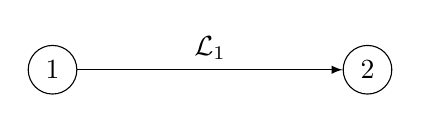
\begin{tikzpicture}

\def \width{4cm}
\def \margin{4mm}

\node (1) [draw, circle] at (0,0) {$1$};
\node (2) [draw, circle] at ({\width},0) {$2$};
\draw[->, >=latex] (1) -- node[above] {$\mathcal{L}_1$} (2);

\end{tikzpicture}


%\end{document}
    \caption{The simple \emph{two-node}\index{network!two-node} transmission network of two nodes and one line.}
    \label{fig:twonodes}
\end{figure}
\begin{example}[Two-node network]\label{exa:twonodenetwork}
A very simple transmission network is one with just two nodes, and a single line connecting them. This \emph{two-node network}\index{network!two-node} is drawn in Figure \ref{fig:twonodes}.
Although real networks are much bigger, this example is useful to illustrate some of the concepts introduced in this chapter.
\begin{align*}
    \intertext{We have:}
    \mathcal{N}&=\{1,2\} \text{ and}\\
    \mathcal{L}&=\{\mathcal{L}_1\}\text{ with }\mathcal{L}_1=(1,2). \\
    \intertext{Since $n=2$ and $m=1$, $\mat{K}$ is a $2\times 1$ matrix:}
    \mat{K} &= \begin{pmatrix}
    1 \\
    -1
    \end{pmatrix}.
\end{align*}
\end{example}

\begin{figure}[h]
    \centering
    %\documentclass{standalone}\usepackage{tikz}\begin{document}


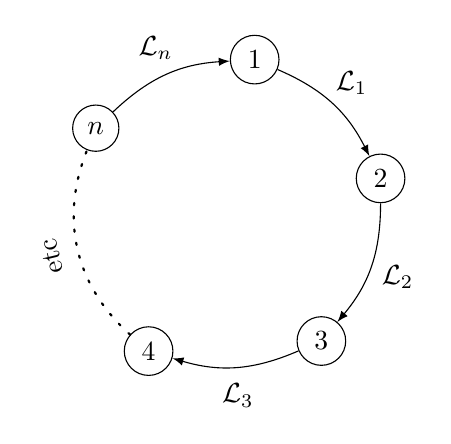
\begin{tikzpicture}

\def \margin{4mm}
\def \radius {2cm}
\def \labelsep {3mm}
\def \dotsep {.4mm}
\def \bend {20}
\def \dotbend {35}
\def \dotmargin {15}

\def \n {4}

\foreach \i in {1,...,\n}
{
  \node (\i) [draw,circle] at ({180 - 360/(\n + 1.4) * (\i +.5)}:\radius) {\i};
}

\foreach \i [remember=\i as \lasti (initially 1)] in {2,...,\n}
{
  \draw[->, >=latex] (\lasti) to[bend left=\bend] (\i);
  \node at ({180 - 360/(\n + 1.4) * (\i +.5 - .5)}:{\radius + \labelsep}) {$\mathcal{L}_\lasti$};
  \node at ({0 + (360/(\n + 1.4) * (\i +.5 - .5))}:{\radius + \labelsep}) {\hphantom{$\mathcal{L}_\lasti$}};
}

\node (n) [draw, circle] at ({180 - 360/(\n + 1.4) * (0 +.5)}:\radius) {$n$};

\draw[->, >=latex] (n) to[bend left=\bend] (1);
\node at ({180 - 360/(\n + 1.4) * (1 +.5 - .5)}:{\radius + \labelsep}) {$\mathcal{L}_n$};

\node[rotate=(( - 360/(\n + 1.4) * (\n/2 + .5)) - 90)] at ({(-360/(\n + 1.4) * (\n/2 + .5))}:{\radius + \labelsep}) {etc};

\draw[thick,line cap=round,loosely dotted, >=latex] (\n) to[bend left=\dotbend] (n);
%\draw[thick,line cap=round,loosely dotted] ({360/(\n + 1.4) * (0 +.5) - \dotmargin}:{\radius - \dotsep}) arc ((360/(\n + 1.4) * (0 +.5))+360 - \dotmargin:(360/(\n + 1.4) * (4 +.5)) + \dotmargin:\radius - \dotsep);


%\draw[color=red] (0:\radius) arc (0:360:\radius);

%\node (1) [draw, circle] at (0,0) {$1$};
%\node (2) [draw, circle] at ({\width},0) {$2$};
%\draw[->, >=latex] (1) -- node[above] {$\mathcal{L}_1$} (2);

\end{tikzpicture}


%\end{document}
    \caption{The \emph{$n$-loop}\index{network!$n$-loop} transmission network with $n$ nodes and $n$ lines.}
    \label{fig:nloopnetwork}
\end{figure}

\begin{example}[Loop network]\label{exa:nloopnetwork}
A less trivial transmission network is the \emph{$n$-loop network}\index{network!$n$-loop}, shown in Figure \ref{fig:nloopnetwork}. It consists of $n$ nodes, connected in a circular fashion (using $n$ lines).

Note that this network is 2-edge connected, meaning that the network remains connected when any edge is removed. (Although removing \emph{any} two lines will disconnect the network.)
\begin{align*}
    \intertext{We have:}
    \mathcal{N}&=\{1,\dots,n\}=\range{n} \text{ and}\\
    \mathcal{L}&=\{\mathcal{L}_1,\dots,\mathcal{L}_n\}\text{ with }\mathcal{L}_i=(i,i+1)\text{ for }1 \leq i < n\text{ and }\mathcal{L}_n=(n,1). \\
    \intertext{Since $m=n$, $\mat{K}$ is an $n\times n$ matrix:}
    \mat{K} &= \begin{pmatrix}
    1 &  & &  & &  -1 \\
    -1 &  1 &  &   &   &   \\
      & -1 &  1 &  &       & \\
      &   &  \ddots & \ddots  &   &   \\
      &   &   & & 1 &    \\
      &   &  &  & -1 &      1  \\
    \end{pmatrix}.
\end{align*}
\emph{(All unspecified elements are 0).}

Note that the \emph{columns} of $\mat{K}$ correspond to the lines of the network.
\end{example}

\begin{figure}
    \centering
    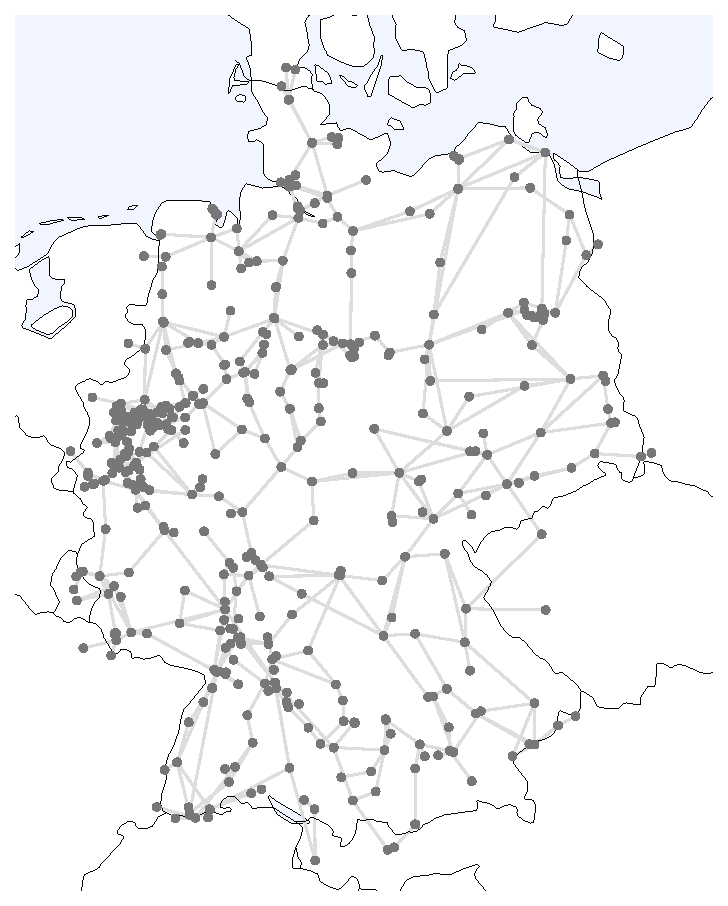
\includegraphics[width=.5\textwidth]{img/scigrid_boring.pdf}
    \caption{The $n=489$ buses and $m=695$ lines of the SciGRID network. A description of this dataset is given in Part II.}
    \label{fig:scigrid}
\end{figure}
\begin{example}[SciGRID Germany]\label{exa:scigridnetwork}
In Part II, we will apply our theory to the SciGRID dataset, which contains the network shown in Figure~\ref{fig:scigrid}. This network is much more realistic than the previous examples, as it is based on the real-world structure of the transmission network in Germany. 

It is common for transmission networks to have a well-connected `core', with some branches out of the core towards the outer regions of the network. This means that in general, $m>n$.

Indeed, in this network we have $n=489$ and $m=695$. The vertex-edge incidence matrix $\mat{K}$ has dimensions $489 \times 695$, and is \emph{sparse}: most entries are zero.

It is important to note that this is only a \emph{section} of the actual transmission network of continental Europe, which is highly connected among different countries. As we will discuss in Section \ref{sec:constructingdataset}, accurate datasets of continental Europe do exist, but they are hard to obtain and analyse.
%Because the laws of physics have no notion of national borders, we would 
%As far as the laws of physics are concerned, taking the subset of lines within Germany is almost as arbitrary as, say, the subset of lines above a certain latitude.
\end{example}
\section{Power grid state}
The \emph{state} of the network describes how the transmission network is being used (the (real and reactive) power injected at each node, and the voltage magnitudes) and how the electric circuit responds (voltage angles and (complex) line currents). More precisely, we use three physical quantities used in AC circuit analysis to describe the grid state:
\begin{definition}\label{def:gridstate}
A \emph{grid state}\index{grid!state} of an $(n,m)$-grid structure is defined as a tuple $(\mat{S}, \mat{V}, \mat{I})$, where
\begin{itemize}
    \item $\mat{S} \in \mathbb{C}^n$ is the \emph{complex power injection vector};
    \item $\mat{V} \in \mathbb{C}^n$ is the \emph{bus voltage vector};\todo{U instead of V? Not common in lit}
    \item $\mat{I} \in \mathbb{C}^m$ is the \emph{line current vector}. (Currents are directed along digraph edges.)
\end{itemize}
\end{definition}
\towrite{Uitleg van AC circuits, real and reactive power, complexe grootheden, etc mist nog. In Hoofdstuk 3 van \cite{VonMeier2006} is het erg duidelijk uitgelegd.}
\section{State validity}

Given an $(n,m)$-grid structure $((\mathcal{N},\mathcal{L}),\mat{K},\mat{\eta})$, only some states are physically possible. A state that satisfies Kirchoff's Laws and Ohm's Law will be called \emph{valid}. Of course, since we are studying a real-world system, we are mainly interested in states that are valid, or at least close to being valid (in the sense of \emph{DC-valid}, see Section \ref{DCapproximation}).

\subsection{Circuit representation}
An $(n,m)$-grid structure $((\mathcal{N},\mathcal{L}),\mat{K},\mat{\eta})$ represents an electrical circuit, consisting of impedances and AC sources. A \emph{valid} grid state $(\mat{S}, \mat{V}, \mat{I})$ corresponds to a physical state of the circuit.
From the mathematical structure, we will construct the corresponding electric circuit in two layers, as follows:

In the first layer, each node $i$ in $\mathcal{N}$ becomes a node in the circuit. The value of $\mel{V}_i$ is the electric potential of that node, relative to ground.

A line $\mathcal{L}_k=(i,j)$ is modelled as an impedance element\footnote{complex-valued resistor} (\inlineres) with admittance $\mel{\eta}_k$ between the two nodes $i$ and $j$. The value of $\mel{I}_k$ is the current flowing through the impedance from $i$ to $j$.\todo{check sign}

See Figure \ref{fig:KVLcircuit} for the first constructed layer. This is not the final circuit: we have not yet added generators and loads to the circuit! Also, the transmission lines have no return wire. This means that there is no closed loop between two nodes, and therefore no energy can be transmitted.

To construct the second layer, we add a new component to each node $i \in \mathcal{N}$, which can be seen as the collection of AC sources (generators) and impedances (loads), connected in parallel between the node and ground. The exact way that loads and generators are connected to the node is not important,\footnote{This would be a circuit comprising the medium and low-voltage networks connected to the node, including every generator, fridge and phone charger that it serves. This is a common (and necessary) abstraction in power grid analysis.} so we will simply state that this component:
\begin{itemize}
    \item sustains a potential difference (which is $\mel{V}_i$);\footnote{In physical systems, the \emph{operating voltage} $|\mel{V}_i|$ (remember that $\mat{V}$ is complex) can be controlled by power plant operators by adjusting excitation current of a generator. The \emph{phase angle} $\theta_j=\Arg(V_j)$ can be controlled by adjusting the amount of energy (steam) supplied to a generator.

    Both methods are an indirect form of control,
    %and the effects are very complex in nature, since the operating voltage and phase angle of one node are inherently linked to that of 
	which also affects    
    all other nodes in the network. In fact, \emph{maintaining} a constant operating voltage and phase angle is a complicated task, requiring continuous adjustments to generator operation. Section 4.3 of \cite{VonMeier2006} covers this topic in more detail.}
    \item either supplies or draws a current, such that the amount of power generated or consumed by the component equals $\mel{S}_i$ (when $\mel{S}_i$ is positive or negative, respectively).
\end{itemize}
We will call this aggregation of generators and loads a \define{power injector} (\inlineac).

Each power injector is connected to a node on one end, and to a ground terminal on the other. In electric circuit theory, a ground terminal represents a direct connection to a universal ground: the `zero' reference of electric potential. One could say that between two different ground terminals, there exists a zero-impedance link connecting the two.
We now have a simple closed circuit between any two nodes connected by a transmission line, consisting of a power injector for the first node, an impedance between the two nodes, a power injector for the second node and a ground link back to the first node.

The complete, two-layer model is shown in Figure \ref{fig:KVLcircuitside}.

\towrite{Justify conductive ground wire in a 3-phase system}

\begin{figure}
    \centering
    \begin{adjustbox}{width=.6\textwidth}
    % By Fons van der Plas
% Based on "Interaction diagram" by Pascal Seppecher, which in turn is based on a diagram from Marco Miani.

%\documentclass[border=5mm]{standalone}\usepackage{tikz}\usepackage[european,siunitx]{circuitikz}\usepackage{amsmath,amssymb}\usetikzlibrary{positioning}\newcommand{\mat}[1]{\ensuremath{\boldsymbol{\mathrm{#1}}}}\newcommand{\mel}[1]{\ensuremath{{\mathrm{#1}}}}\newcommand{\phym}[1]{\ensuremath{\mathsf{#1}}}\begin{document}

\newcommand{\yslant}{0}
\newcommand{\xslant}{0}
\begin{circuitikz}[scale=1.1,every node/.style={minimum size=8mm},on grid]
\ctikzset{label/align = rotate}
	\draw[black, loosely dotted, thick] (0,.3) rectangle (10,7);
	
    % Top level
	\begin{scope}[
		yshift=0,
		every node/.append style={yslant=\yslant,xslant=\xslant},
		yslant=\yslant,xslant=\xslant
	]
	    \coordinate[](1hv) at (1,2);
	    \coordinate[](ihv) at (5,3);
	    \coordinate[](jhv) at (9,3);
	    \coordinate[](2hv) at (3.2,6);
	    
	    \coordinate[](xhv) at (10,3.7);
	    \coordinate[](yhv) at (10,2.2);
	    
	    \coordinate[](thv) at (0.5,.3);
	    \coordinate[](uhv) at (0,2.3);
	\end{scope}
    

	
	% HV level
	\begin{scope}[
		yshift=0,
		every node/.append style={yslant=\yslant,xslant=\xslant},
		yslant=\yslant,xslant=\xslant
	]
		
			
		\draw[] (1hv) to [R,l_=$\mel{Y}_{1,i}$, *-*] (ihv);
		\draw[thick] (jhv) to [R,l=$\mel{Y}_{i,j}$, semithick, *-*] (ihv);
		\draw[] (2hv) to [R,l_=$\mel{Y}_{2,i}$, *-*] (ihv);
		
		\draw[] (jhv) to [] (xhv);
		\draw[] (jhv) to [] (yhv);
		\draw[] (thv) to [] (1hv);
		\draw[] (uhv) to [] (1hv);
		
		\draw[fill=black]  
			(1hv) node[anchor=south] {$\mel{V}_1$}
			(ihv) node[anchor=south] {$\mel{V}_i$}
			(jhv) node[anchor=south] {$\mel{V}_j$}
			(2hv) node[anchor=south] {$\mel{V}_2$};
		
	\end{scope}
	
	
\end{circuitikz}
%\end{document}
    \end{adjustbox}
    \caption{A section of a transmission network, showing the line $(i,j)$. Two more nodes, both connected to $i$, are also shown. Note that this is only one layer of the electric circuit used in the model. In the full model (Figure \ref{fig:KVLcircuitside}), each transmission line forms a closed circuit, allowing current to flow.}
    \label{fig:KVLcircuit}
\end{figure}

%(\protect{\makebox[\width]{\raisebox{-1mm}{\begin{circuitikz}\ctikzset{bipoles/length=7mm}\draw[] (0,0) to[sV] (1,0);\end{circuitikz}}}})
\begin{figure}
    \centering
    \begin{adjustbox}{width=.9\textwidth}
    % By Fons van der Plas
% Based on "Interaction diagram" by Pascal Seppecher, which in turn is based on a diagram from Marco Miani.

%\documentclass[border=5mm]{standalone}\usepackage{tikz}\usepackage[european,siunitx]{circuitikz}\usepackage{amsmath,amssymb}\usetikzlibrary{positioning}\newcommand{\mat}[1]{\ensuremath{\boldsymbol{\mathrm{#1}}}}\newcommand{\mel}[1]{\ensuremath{{\mathrm{#1}}}}\newcommand{\phym}[1]{\ensuremath{\mathsf{#1}}}\begin{document}


\newcommand{\yslant}{.4}
\newcommand{\xslant}{-.7}
\begin{circuitikz}[scale=1.1,every node/.style={minimum size=8mm},on grid]
\ctikzset{label/align = rotate}

    % Ground level
	\begin{scope}[
		yshift=-120,
		every node/.append style={yslant=\yslant,xslant=\xslant},
		yslant=\yslant,xslant=\xslant
	]
	    \coordinate[](1gnd) at (1,2);
	    \coordinate[](ignd) at (5,3);
	    \coordinate[](jgnd) at (9,3);
	    \coordinate[](2gnd) at (3.2,6);
	    
	    \coordinate[](xgnd) at (10,3.7);
	    \coordinate[](ygnd) at (10,2.2);
	    
	    \coordinate[](tgnd) at (0.5,0.3);
	    \coordinate[](ugnd) at (0,2.3);
	\end{scope}
	
	
	
    % Top level
	\begin{scope}[
		yshift=0,
		every node/.append style={yslant=\yslant,xslant=\xslant},
		yslant=\yslant,xslant=\xslant
	]
	    \coordinate[](1hv) at (1,2);
	    \coordinate[](ihv) at (5,3);
	    \coordinate[](jhv) at (9,3);
	    \coordinate[](2hv) at (3.2,6);
	    
	    \coordinate[](xhv) at (10,3.7);
	    \coordinate[](yhv) at (10,2.2);
	    
	    \coordinate[](thv) at (0.5,.3);
	    \coordinate[](uhv) at (0,2.3);
	\end{scope}
    

	% Ground level
	\begin{scope}[
		yshift=-120,
		every node/.append style={yslant=\yslant,xslant=\xslant},
		yslant=\yslant,xslant=\xslant
	] 
	    \fill[white,fill opacity=.7] (0,.3) rectangle (10,7); % Opacity
		% The frame
		\draw[black, loosely dotted, thick] (0,0.3) rectangle (10,7);
		
		
		
		\draw[] (1gnd) to[short,*-*] (ignd) node[ground]{};
		\draw[thick] (jgnd) to[short,*-*] (ignd);
		\draw[] (2gnd) to[short,*-*] (ignd);
		
		\draw[] (jgnd) to [] (xgnd);
		\draw[] (jgnd) to [] (ygnd);
		\draw[] (tgnd) to [] (1gnd);
		\draw[] (ugnd) to [] (1gnd);
		
		 % Level title
		\fill[black]
			(0.2,6.5) node[right, scale=1] {\textbf{Ground}}	
			(5.1,1.9);
	\end{scope}
	
	% Vertical lines
	\draw[](1gnd) to[sV] (1hv);
	\draw[thick](ignd) to[sV, semithick] (ihv);
	\draw[thick](jgnd) to[sV, semithick] (jhv);
	\draw[](2gnd) to[sV] (2hv);
	
	
	\begin{scope}[
		yshift=0,
		every node/.append style={yslant=\yslant,xslant=0},
		yslant=\yslant,xslant=0
	]
	\draw[thick, blue, ->] (3.9,.8) arc (180:-170:1);
	\fill[black]
			(4.9,.8) node[blue, scale=1] {KVL}; 
	\end{scope}
	
	
	
	% HV level
	\begin{scope}[
		yshift=0,
		every node/.append style={yslant=\yslant,xslant=\xslant},
		yslant=\yslant,xslant=\xslant
	]
		% The frame:
		\fill[white,fill opacity=.7] (0,.3) rectangle (10,7); % Opacity
		\draw[black, loosely dotted, thick] (0,.3) rectangle (10,7);
		
			
		\draw[] (1hv) to [R,l_=$\mel{Y}_{1,i}$, *-*] (ihv);
	    \draw[thick] (jhv) to [R,l=$\mel{Y}_{i,j}$, semithick, *-*] (ihv);
		\draw[] (2hv) to [R,l_=$\mel{Y}_{2,i}$, *-*] (ihv);
		
		\draw[] (jhv) to [] (xhv);
		\draw[] (jhv) to [] (yhv);
		\draw[] (thv) to [] (1hv);
		\draw[] (uhv) to [] (1hv);
		
		\draw[fill=black]  
			(1hv) node[anchor=south] {$\mel{V}_1$}
			(ihv) node[anchor=south] {$\mel{V}_i$}
			(jhv) node[anchor=south] {$\mel{V}_j$}
			(2hv) node[anchor=south] {$\mel{V}_2$};
		 % Level title
		\fill[black]
			(0.2,6.5) node[right, scale=1] {\textbf{High-Voltage}}; 
	\end{scope}
	\draw[orange, rounded corners=3mm, dashed, thick] ($(ihv)-
	(1,1)$) rectangle ($(ihv) + (1,1)$);
	\node[orange,above] at ($(ihv) + (0,1)$){KCL};
	
	
\end{circuitikz}
%\end{document}
    \end{adjustbox}
    \caption{
    The electric model of the transmission network, showing the line $(i,j)$ and two other nodes. A node is represented by a single component (\inlineac), which is the aggregation of all generators and loads connected to that node. A transmission line is modelled as an impedance (\inlineres), a complex-valued resistor. The ground 'wires' have zero resistance. \protect\newline
    \textbf{KVL} is applied to each \textbf{line}, by traversing the loop drawn in blue.\protect\newline
    \textbf{KCL} is applied to each \textbf{node}, by summing all currents entering and leaving the orange area.}
    \label{fig:KVLcircuitside}
\end{figure}

\subsection{Kirchoff's Voltage Law (KVL) \& Ohm's Law}
For each line $\mathcal{L}_k=(i,j)$, we can apply Kirchoff's Voltage Law to the loop ``ground $\rightarrow$ $i$ $\rightarrow$ $j$ $\rightarrow$ ground'', as shown in Figure \ref{fig:KVLcircuitside}. This gives us:
$$\mel{V}_i + \Delta \mel{V}_k + -\mel{V}_j = 0,$$
where $\Delta \mel{V}_k$ is the electric potential of the line impedance. This potential relates to the line current according to Ohm's Law:
$$\mel{I}_k = \Delta \mel{V}_k \cdot \mel{\eta}_k = (\mel{V}_j - \mel{V}_i) \cdot \mel{\eta}_k.$$
Since the $k$th column of $\mat{K}$ (which corresponds to the line $\mathcal{L}_k=(i,j)$) has exacly two non-zero entries: $\mel{K}_{i,k}=1$ and $\mel{K}_{j,k}=-1$, we can write:
$$\mel{I}_k = (\mel{V}_j - \mel{V}_i) \cdot \mel{\eta}_k = -(\mel{K}^*{V})_{k}\mel{\eta}_k.$$
This holds for every $k \in \range{m}$, and this system of equations can be written compactly as:
$$\mat{I} = i\diag(i\mat{\eta})\mat{K}^*\mat{V}$$
\towrite{Written in this form, we see that when $i\bm{\eta}, \mathbf{C}$ and $\mathbf{V}$ are purely real, then $\mathbf{I}$ is purely imaginary. Physically, this means that line current is always $90\si{\degree}$ out of phase with voltage differences. When phase angles are small, and voltage magnitude is constant, then these differences are almost purely imaginary.}
\todo{Writing node voltages in a circuit implies that already KVL holds.}
\subsection{Kirchoff's Current Law (KCL)}
Using KVL and Ohm's Law, we found a relation between line current and node voltages. We can use KCL to relate the power injection to currents leaving and entering a bus.

We apply KCL to every high-voltage node in the electric circuit, as shown in Figure \ref{fig:KVLcircuitside}. For a bus $i \in \range{n}$, Kirchoff's Current Law states:
\[
\left[ \text{\textit{sum of currents leaving the node}}\right] \, - \, \left[\text{\textit{sum of currents entering the node}}\right] = 0.
\]
These currents are the currents of lines incident at the bus, together with the current `generated or consumed' by the power injector. Complex power is given by:
\[
\phym{S} = \conj{\,\phym{I}\,}\phym{V}.
\]
In our case, $\phym{I}$ is the current that we are looking for, flowing from the ground node to the high-voltage node at $i$, and $\phym{V}$ is the potential difference between the high-voltage node and ground, which is $\mel{V}_i$. The amount of power generated or consumed is given by the grid state: $\phym{S}=\mel{S}_i$. The current through the power injector is now given by $\conj{\mel{S}_i \mel{V}_i^{-1}}$.

The $i^{\text{th}}$ row of $\mat{K}$ corresponds to the bus $i$, and its entries are $1$ for lines leaving $i$, and $-1$ for lines entering $i$. This allows us to write the sum of currents in a compact way:
\[
\conj{\mel{S}_i \mel{V}_i^{-1}} + (\mel{K}\mel{I})_i = 0.
\]
Taking the complex conjugate and multiplying both sides by $\mel{V}_i$ gives $\mel{S}_i + \conj{(\mel{K}\mel{I})}_i \mel{V}_i = 0$ for each $i \in \range{n}$, or in matrix form:
$$\mat{S}+\conj{(\mat{K} \mat{I})}\pointwise \mat{V} = \mat{0}.$$
(The symbol $\pointwise$ denotes \emph{point-wise} multiplication.)
\subsection{Validity conditions}
Instead of \emph{requiring}\footnote{\cite{Slepian1968} gives an \emph{axiomatic} formulation of circuit theory.} the circuits laws to hold, we define them as an \emph{optional property} of the grid state.
\begin{definition}\label{def:statevalidity}
Given an $(n,m)$-grid structure $((\mathcal{N},\mathcal{L}),\mat{K},\mat{\eta})$, a grid state $(\mat{S}, \mat{V}, \mat{I})$ is \define{valid} if it satisfies the \define{KVL-Ohm equality}:
\begin{align}\label{eq:KVLOhmeq}
    \mat{I} = i\diag(i\mat{\eta})\mat{K}^*\mat{V} \tag{KVL-Ohm}
\end{align}
and the \define{KCL equality}:
\begin{align}\label{eq:KCLeq}
    \mat{S}+\conj{(\mat{K} \mat{I})}\pointwise \mat{V} = \mat{0}. \tag{S-KCL}
\end{align}
\end{definition}
\begin{remark}
In physical terms, the \emph{KVL-Ohm equality} states:
\begin{gather*}
    \textit{Each line $\mathcal{L}_k=(i,j)$ satisfies Ohm's Law ($\phym{I=VY}$), where:} \\
    \phym{I}=\mel{I}_k, \qquad \phym{V}=\mel{V}_{i} - \mel{V}_j, \qquad \phym{Y}=\mel{\eta}_k \nonumber
\end{gather*}
and the \emph{KCL equality} states:
\begin{gather*}
    \textit{At each node $i$, the sum of power injected at the node, $\mel{S}_i$}, \\
    \textit{and power injected from the grid, must equal $0$.} \nonumber
\end{gather*}
\end{remark}

\begin{proposition}
Given a grid structure and state as in Definition \ref{def:statevalidity}, the following are equivalent:
\begin{enumerate}[label=\roman*.]
    \item The grid state is valid.
    \item The grid state satisfies (\ref{eq:KVLOhmeq}) and (\ref{eq:KCLeq}).
    \item The grid state satisfies (\ref{eq:KVLOhmeq}), and each node $i$ satisfies the \define{node flow equation}, also called the \define{power mismatch equation}:
    \begin{empheq}[box=\fbox]{gather}
        \mel{S}_i = i\sum_{j=1}^{n} \conj{\mel{L}}_{i,j} |\mel{V}_i| |\mel{V}_{j}| e^{i(\theta_i - \theta_j)}\quad\quad\text{for each $i \in \range{n}$,}\label{eq:nodefloweq}\\
        \text{where }\mat{L}=\mat{K} \diag(i\mat{\eta}) \mat{K}^*
    \end{empheq}
    and $\mat{\theta} \in \mathbb{R}^n$ is the vector of \emph{voltage angles}, \ie $\theta_j=\Arg(V_j)$ (the principle argument of $\mel{V}_j$). We call $\mat{L}$ the \define{nodal susceptance matrix} \citep{Ronellenfitsch2017}.
\end{enumerate}

\end{proposition}
\begin{remark}
Note that (\ref{eq:nodefloweq}) does not depend on $\mat{I}$. This means that a valid state is uniquely determined by $\mat{S}$ and $\mat{V}$, since $\mat{I}$ can be computed from $\mat{V}$ using (\ref{eq:KVLOhmeq}).
\end{remark}


\begin{remark}
Writing in real and imaginary components, we get the node flow equations for real and reactive power for each node $i \in \range{n}$:
\begin{align}
    %\mel{S}_i &= \sum_{j=1}^{n} (\Re(\conj{\mel{M}}_{i,j})+i\Im(\conj{\mel{M}}_{i,j})) |\mel{V}_i| |\mel{V}_{j}| (\cos(\theta_i - \theta_j)+i\sin(\theta_i - \theta_j)) \\
    %\phym{P}=\Re (\mel{S}_i) &= \sum_{j=1}^{n} |\mel{V}_i| |\mel{V}_{j}| \Big[\Re(\mel{M}_{i,j})\cos(\theta_i - \theta_j)+\Im(\mel{M}_{i,j})\sin(\theta_i - \theta_j)\Big]
    \phym{P}=\Re (\mel{S}_i) &= \sum_{j=1}^{n} |\mel{V}_i| |\mel{V}_{j}| \Big[\Im(\mel{L}_{i,j})\cos(\theta_i - \theta_j)-\Re(\mel{L}_{i,j})\sin(\theta_i - \theta_j)\Big]
    \label{eq:realreactivenodefloweqreal}
    \\
    %\phym{Q}=\Im (\mel{S}_i) &= \sum_{j=1}^{n} |\mel{V}_i| |\mel{V}_{j}|\Big[\Re(\mel{M}_{i,j})\sin(\theta_i - \theta_j)-\Im(\mel{M}_{i,j})\cos(\theta_i - \theta_j)\Big]
    \phym{Q}=\Im (\mel{S}_i) &= \sum_{j=1}^{n} |\mel{V}_i| |\mel{V}_{j}|\Big[\Im(\mel{L}_{i,j})\sin(\theta_i - \theta_j)+\Re(\mel{L}_{i,j})\cos(\theta_i - \theta_j)\Big]
    \label{eq:realreactivenodefloweqreactive}
\end{align}
In literature on the subject, the node flow equation is often given in this form. The summands in the expression above are essentially the two-dimensional rotation matrix of angle $\theta_i - \theta_j$, applied to the vector $(\Re(i \conj{\mel{L}}_{i,j}), \Im(i \conj{\mel{L}}_{i,j}))^*$.

We will later study so called \emph{DC-valid} grid structures, where the values of $\mat{L}$ are real. If so, (\ref{eq:realreactivenodefloweqreal}) simplifies to:
\begin{align*}
    \phym{P}=\Re (\mel{S}_i) &= \sum_{j=1}^{n} \Re(\mel{L}_{i,j}) |\mel{V}_i| |\mel{V}_{j}| \sin(\theta_j - \theta_i).
\end{align*}
(Notice that we flipped $\theta_i$ and $\theta_j$.)
This tells us that in a network of just two nodes and one line with purely imaginary admittance, \todo{move to separate Example} the amount of real power transmitted is proportional to $\sin (\theta_2-\theta_1)$.\footnote{The quantity $\theta_2 - \theta_1$ is called the \define{power angle} of the transmission line, a common measure of the amount of power being transmitted. As discussed in Section \ref{gridstability}, a power angle greater than $45\si{\degree}$ will cause the nodes to lose synchronicity, making power transmission between the two nodes impossible. For long lines (over $100\si{\kilo\meter}$), this \define{stability limit} places an upper limit on the amount of power that a line can transmit. For shorter lines, the \emph{thermal limit} dominates.}


\end{remark}

\begin{proof}
(i) $\iff$ (ii) is true by definition.

Suppose the grid state satisfies (\ref{eq:KVLOhmeq}). We have
\begin{align*}
    \mat{S}+\conj{(\mat{K} \mat{I})}\pointwise \mat{V} &=\\
    \mat{S}+\conj{(i\mat{K} \diag(i\mat{\eta}) \mat{K}^* \mat{V})} \pointwise \mat{V} &= \\
    \mat{S}+\conj{(i\mat{L} \mat{V})} \pointwise \mat{V} &= \mat{0}
\end{align*}\todo{is this Newton's heat equation with M the discrete Laplacian?}
iff for each $i\in\range{n}$
\begin{align*}
    \mel{S}_i &= -\conj{\left(\sum_{j=1}^{n} i\mel{L}_{i,j} \mel{V}_{j}\right)} \mel{V}_i \\
    &= -\left(\sum_{j=1}^{n} -i\conj{\mel{L}}_{i,j} \conj{\mel{V}}_{j}\right) \mel{V}_i \\
    &= i\sum_{j=1}^{n} \conj{\mel{L}}_{i,j} \mel{V}_i \conj{\mel{V}}_{j} \\
    &= i\sum_{j=1}^{n} \conj{\mel{L}}_{i,j} |\mel{V}_i| e^{i\theta_i} |\mel{V}_{j}| e^{-i\theta_j} \\
    &= i\sum_{j=1}^{n} \conj{\mel{L}}_{i,j} |\mel{V}_i| |\mel{V}_{j}| e^{i(\theta_i - \theta_j)},
\end{align*}
proving (ii) $\iff$ (iii).
\end{proof}

\section{Power Flow}
In the previous section, we derived a fundamental result: the \emph{node flow equation} (\ref{eq:nodefloweq}).
Recall from Section \ref{sec:powerflow} that the \emph{Power Flow problem} entails the following:
\begin{empheq}{gather*}
    \text{\emph{Given the production or consumption at each node,}}\\
    \text{\emph{\textbf{find the current flowing through each line.}}}
\end{empheq}
In the context of our electric model, this translates to:
\begin{empheq}{gather*}
    \text{\emph{Given an $(n,m)$-grid structure $((\mathcal{N},\mathcal{L}),\mat{K},\mat{\eta})$, and a power injection $\mat{S}$, }}\\
    \text{\emph{\textbf{find $\mat{V}$ and $\mat{I}$ such that $(\mat{S}, \mat{V}, \mat{I})$ is a valid state.}}}
\end{empheq}

It turns out that the easiest way to solve this problem is to solve the node flow equation, obtaining $\mat{V}$. Once $\mat{V}$ is known, one can easily compute $\mat{I}$ using \ref{eq:KVLOhmeq}, giving a state $(\mat{S}, \mat{V}, \mat{I})$ that is valid by construction.

The node flow equation is a system of non-linear equations, and no closed-form solution is known to exist in general. Fortunately, solving the node flow equation is essentially a root-finding problem. This means that well-established techniques, such as the Newton-Raphson algorithm, can be used to find a numerical solution.

The only difficulty lies in the \emph{number of unknowns} ($2n$ real numbers\footnote{Actually, the voltage angle $\theta$ of one bus (the \emph{slack bus}) is usually fixed to $0$, since \ref{eq:nodefloweq} only depends on \emph{differences} in voltage angles. We then have $2n-1$ unknowns.}) and finding an \emph{initial value} that converges to the solution. When studying the evolution of the grid state over time, we can use the solution of a previous iteration as initial value. In general, however, we need to come up with an initial guess.

The classical approach is to use the \define{flat start} as initial value: all voltage angles are set to $0$, and magnitudes are all set to the same value (say, $380 \, \si{\kilo\volt}$). For small networks, the Newton-Raphson algorithm then converges to a valid state, with small power angles between lines, and voltage magnitudes close to the initial value. For larger networks, however, this initial value rarely converges, and a valid is state can be `maddeningly difficult to obtain' \citep{Overbye2004}. 

Instead, a common approach is to approximate the grid structure and to linearises the laws of physics. The more approximations that we make, the easier it is to find a solution. A particular combination of approximations is known as the \emph{DC approximation}, in which case a \emph{closed-form} solution always exists, known as the \emph{Linear Power Flow}. For accurate power flow analysis, this solution is then used as initial value for the original system of equations. In this thesis, however, we will only use the solution of the Linear Power Flow, as it is easier to compute and analyse. This is common practice when studying \emph{cascading failures} \citep{Nesti2018emergentfailures, Ronellenfitsch2017, Purchala}.
\section{DC approximation}\label{DCapproximation}
`DC approximation' is a name given to a collection of assumptions/approximations, described below. The name `DC' refers to the approximation that the network is \emph{decoupled}. Unlike the abbreviation might suggest (DC usually stands for `Direct Current'), the power grid is still modelled as an AC (Alternating Current) network. The first version of this technique was published by \cite{Scott1974}, allowing the node flow equations to be solved efficiently using the computational power available at that time.\footnote{Their method does solve the actual node flow equation, but they optimised the iterative root-finding process by \emph{approximating the Jacobian}.}

Compare the following with Definitions \ref{def:gridstructure} and \ref{def:gridstate}.
\begin{definition}\label{def:DCaproximated}
Suppose $((\mathcal{N},\mathcal{L}),\mat{K},\mat{\eta})$ is an $(n,m)$-grid structure.
\begin{itemize}
    \item If $i\mat{\eta} \in \mathbb{R}^m \subseteq \mathbb{C}^m$  (\ie $\mat{\eta}$ has purely imaginary values) then the grid structure \emph{satisfies the DC approximation}\index{DC approximation!structure}.
    \footnote{\cite{Nesti2018emergentfailures} write $\beta=i\mat{\eta}$. Transmission line impedance ($\phym{Z=R+iX}$) is dominated by inductance, which is positive reactance  ($\phym{X}$). Resistance ($\phym{R}$) is always positive for passive components. Therefore, $\phym{Z}$ lies in the top-right quadrant of $\mathbb{C}$. Then the admittance, $\phym{Y=1/Z=G+iB}$, lies in the bottom-right quadrant of $\mathbb{C}$. In the DC approximation, line conductance ($\phym{G}$) is neglected, so ($\phym{Y=iB}$ with $\phym{B}<0$). Therefore, $\beta_k=i\eta_k=i\phym{Y}=-\phym{B}>0$ is the \emph{susceptance of line $k$, \textbf{with reversed sign.}}}
\end{itemize}
For a grid state $(\mat{S}, \mat{V}, \mat{I})$ on the structure:
\begin{itemize}
    \item If $\mat{S} \in \mathbb{R}^n \subseteq \mathbb{C}^n$ then the grid state \emph{satisfies the DC approximation}\index{DC approximation!state}. (Note that $\mat{V}$ and $\mat{I}$ need not be real-valued! We are still studying an AC circuit.)
    \item If $\mat{V} \in \mathbb{T}^n \cdot V_{op} \subseteq \mathbb{C}^n$ (\ie $|V_i|=V_{op}$ for each node $i$) for some \define{operating voltage} $V_{op} \in \mathbb{R}_{\geq 0}$, then the grid state admits a \define{flat profile}.

    In the special case $V_{op}=1$, the grid state admits a \define{normalised profile}.
\end{itemize}
\end{definition}
We note that $V_{op}=1$ does not necessarily mean that the transmission network is operating at $1 \, \si{\volt}$, it simply means that the network is operating at exactly \emph{one unit of electric potential} (which could be set to $1 \, \si{\volt}$, but also $380 \, \si{\kilo\volt}$, for example). This unit is known as a \define{power unit} (p.u.).

\towrite{There is no line drop in a DC approximated structure}

Compare the following with Definition \ref{def:statevalidity} and (\ref{eq:nodefloweq}).
\begin{definition}\label{def:approximatestatevalidity}
Given an $(n,m)$-grid structure $((\mathcal{N},\mathcal{L}),\mat{K},\mat{\eta})$ and a grid state $(\mat{S}, \mat{V}, \mat{I})$ that both satisfy the DC approximation. The grid state is \emph{approximately valid} if it satisfies the \emph{approximate KVL-Ohm equality}:
\begin{align}\label{eq:approxKVLOhmeq}
    \mat{I} = i\diag(i\mat{\eta})i\mat{K}^*\mat{\theta}V_{op} \tag{approx. KVL-Ohm}
\end{align}
and the \emph{approximate KCL equality}:
\begin{align}\label{eq:KCLeq}
    \mat{S}+\conj{(\mat{K} \mat{I})} V_{op} = \mat{0}. \tag{approx. S-KCL}
\end{align}
\end{definition}
The approximate KCL equality can be obtained by replacing the $\exp$ function in (\ref{eq:nodefloweq}) by $z \mapsto 1+z$ (the first two terms of the Maclaurin series of $\exp$):
\begin{proposition}\label{prop:approxnodeflow}
Given a grid structure state as in the previous definition, the state is approximately valid if and only if it satisfies the approximate KVL-Ohm equality and each node $i$ satisfies the \emph{approximate node flow equation}\index{node flow equation!approximate}:
\begin{empheq}[box=\fbox]{align}
    \mel{S}_i &= i\sum_{j=1}^{n} \conj{\mel{L}}_{i,j} |\mel{V}_i| |\mel{V}_{j}| (1+i(\theta_i - \theta_j))\quad\quad\text{for each $i \in \range{n}$.}\label{eq:approxnodefloweq}
\end{empheq}
\end{proposition}
\begin{proof}
Suppose the approximate KVL-Ohm equality hold. The approximate node flow equality holds if and only if for each node $i$, we have:
\begin{align*}
\mel{S}_i &= i\sum_{j=1}^{n} \conj{\mel{L}}_{i,j} |\mel{V}_i| |\mel{V}_{j}| (1+i(\theta_i - \theta_j)) \\
    &= i\sum_{j=1}^{n} \mel{L}_{i,j} |\mel{V}_i||\mel{V}_{j}| -  \sum_{j=1}^{n} \mel{L}_{i,j} |\mel{V}_i||\mel{V}_{j}|(\theta_i - \theta_j)\\
    \intertext{We assumed a DC state ($\mel{S}_i \in \mathbb{R}$):}
    &= -\sum_{j=1}^{n} \mel{L}_{i,j} |\mel{V}_i||\mel{V}_{j}|(\theta_i - \theta_j)\\
    &= -\sum_{j=1}^{n} \mel{L}_{i,j} |\mel{V}_i||\mel{V}_{j}|\theta_i + \sum_{j=1}^{n} \mel{L}_{i,j} |\mel{V}_i||\mel{V}_{j}|\theta_j\\
    &= -\theta_i |\mel{V}_i| \sum_{j=1}^{n} \mel{L}_{i,j}|\mel{V}_{j}| + |\mel{V}_i| \sum_{j=1}^{n} \mel{L}_{i,j} |\mel{V}_{j}|\theta_j\\
    \intertext{We assumed a flat profile ($|\mel{V}_i|=|\mel{V}_j|=V_{op}$ for every $i,j \in \range{n}$):}
    &= -\theta_i V_{op}^2 \sum_{j=1}^{n} \mel{L}_{i,j} + V_{op}^2 \sum_{j=1}^{n} \mel{L}_{i,j} \theta_j\\
	&= -\theta_i V_{op}^2 \sum_{j=1}^{n} \conj{\mel{L}}_{i,j} + V_{op}^2 \sum_{j=1}^{n} \mel{L}_{i,j} \theta_j\\
    \intertext{The rows of $\mat{L}$ add up to $0$:}
	&= 0 + V_{op}^2 \sum_{j=1}^{n} \mel{L}_{i,j} \theta_j\\
	&= V_{op}^2 \sum_{j=1}^{n} \mel{L}_{i,j} \theta_j\\
	&= (\conj{\mel{L}}\mel{\theta})_i V^2_{op} \\
	&= \conj{(\mel{K} \diag(i\mel{\eta})\mel{K}^*\mel{\theta})_i} V^2_{op} \\
	&= -\conj{(\mel{K} i\diag(i\mel{\eta})i\mel{K}^*\mel{\theta}V_{op})_i} V_{op} \\
	&= -\conj{(\mel{K} \mel{I})_i} V_{op}
\end{align*}
which is equal to $\mel{S}_i$ if and only if the approximate KCL equality holds.
\end{proof}

\begin{theorem}\label{thm:approxnodeflowlineq}
Suppose that a grid structure and state satisfy the DC approximation and that the state admits a flat, normalised profile. Then the approximated node flow equation is linear and real:
\begin{empheq}[box=\fbox]{align}
    \mat{S} &= \mat{L}\mat{\theta}.\label{eq:approxnodeflowlineq}
\end{empheq}
\end{theorem}

\begin{proof}
In the proof of Theorem \ref{prop:approxnodeflow}, we derived that the approximate node flow equation holds if and only if for each node $i$, we have:
\begin{align*}
    \mel{S}_i = (\conj{\mel{L}}\mel{\theta})_i V^2_{op}.
\end{align*}
Because $\mat{L}$ is real-valued and $V_{op}=1$, we find the result.
\end{proof}
\towrite{Appendix: give a direct formula for $\mathbf{L}$}
\towrite{compute $\mathbf{L}$ for the example networks}
\towrite{give an alternative interpretation of $\mathbf{L}$ or $\mathbf{L}$: discrete laplacian}
\towrite{discuss the kernel of $\mathbf{L}$: it should be the space spanned by $(1,1,\dots,1)^*$, such that the nullity of $\mathbf{L}$ is $1$. This corresponds to the fact that phase angle is a relative quantity. (The state remains (DC-)valid when increasing the phase angle at each node by the same amount. (If $\mathbf{S}=\mathbf{L\theta}$ and $\mathbf{\theta}_0 \in \ker \mathbf{L}$, then $\mathbf{S}=\mathbf{L}(\bm{\theta}+\bm{\theta_0})$.))\\There are two paths to take after this point:\\1: Fix the phase angle of the slack bus (to $0$), which corresponds to taking the ${n-1 \times n-1}$ submatrix of $\mathbf{L}$, I think. \textbf{This is the approach of PyPSA, which might explain small differences in line flow.} \\2: Leave $\mathbf{L}$ as-is, and consider the \emph{Moore-Penrose pseudo-inverse} of $\mathbf{L}$. This is the approach of Nesti et al., which they attribute to 'distributive slack': not fixing a single slack bus.}

%\subsection{Usefulness}
%Real transmission networks do not satisfy the DC approximation and, in general, a DC-valid state is not (physically) valid. Yet, using these two approximations has one important property: the approximated node flow equation becomes \emph{linear}. This has a number of advantages:
%\begin{itemize}
%    \item Solving the Power Flow problem (\ie computing line flows induced by a power injection vector) becomes trivial. As we will see in Section \ref{LPFequations}, \towrite{ugh}
%    \item A linear power flow is crucial for the study of stochastic power injections, since it can be used to transform a probability distribution (like a multivariate normal distribution) without losing its structure.\todo{be specific}
%\end{itemize}

\subsection{Accuracy}
The DC approximation is a useful tool for understanding the complex nature of transmission networks. Therefore, it is crucial to verify that the DC approximation is, in fact, a good approximation, when real-world networks are studied. More precisely, one should ask:
\begin{enumerate}
    \item How close is a DC-valid state to being valid? More precisely, when the approximate node flow equation (\ref{eq:approxnodefloweq}) holds, what is the mismatch between the left hand and right hand side of the node flow equation (\ref{eq:nodefloweq})?
    \item How close are real-world grid structures to satisfying the DC approximation?
    %\item How does modifying a grid structure to satisfy the DC approximation affect the resulting power flow solution?
\end{enumerate}

The first question is answered in Proposition \ref{prop:powermismatchupperbound}, where an upper bound is derived for the power mismatch. It shows that the mismatch is bounded by the \emph{squares} of local differences in phase angles (i.e. $\theta_i - \theta_j$ for line $(i,j)$). \citet{Purchala} have shown that in the Belgian transmission network, all phase differences are below $7 \si{\degree}$, and $94\si{\percent}$ of lines have a phase difference below $2\si{\degree}$.

The second question \todo{SciGRID} \todo{Purchala}

\towrite{acc of DC approx struc vs acc of DC valid state}
\tocite{literature: \cite{Purchala,Overbye2004}}

\begin{lemma}\label{lem:expaprrox}\todo{Move to appendix?}
There exists $K \in \mathbb{R}_{\geq 0}$ such that
\begin{align*}
    |\exp ix - (1 + ix)| = K |x|^2 \qquad \text{for every $-2\pi \leq x \leq 2\pi$}.
\end{align*}
\end{lemma}\todo{Find an upper bound for $K$, $K=0.5$ works}

\begin{proof}
\textbf{A proof using complex analysis}.\footnote{For an introduction, see \cite{GarlingVolIII}.} The complex (entire) function $z \mapsto \exp z$ is defined by the power series
\begin{align*}
    z\mapsto \sum_{k=0}^{\infty} \frac{z^k}{k!} = 1 + z + z^2\left(\frac{z^0}{2!}+\frac{z^1}{3!}+\dots\right)
\end{align*}\todo{$0^0$}
which has infinite radius of convergence, and is continuous on $\mathbb{C}$.

The functions $z \mapsto \frac{1}{z^2}$, $z \mapsto \exp z$ and $z \mapsto 1+z$ are all holomorphic on $\mathbb{C}^*=\mathbb{C} \setminus \{0\}$, and so the function
\begin{align}
    g: \mathbb{C}^* \rightarrow \mathbb{C} \qquad \qquad
    g: z \mapsto \frac{1}{z^2}(\exp z - (1+z))
\end{align}
is holomorphic on $\mathbb{C}^*$, with a removable singularity at $0$. The (unique) extension of $g$ to $\mathbb{C}$ is an entire function, and by construction:
\begin{align*}
    \exp z = 1 + z + z^2g(z)\qquad \text{for each $z \in \mathbb{C}$}.
\end{align*}
Since $g$ is entire, it is continuous on $\mathbb{C}$.
$I=[-i2\pi, i2\pi]$ is a compact subset of $\mathbb{C}$, so $g$ is bounded on $I$, proving the result.
\end{proof}

\begin{proposition}\label{prop:powermismatchupperbound}
Suppose $((\mathcal{N},\mathcal{L}),\mat{K},\mat{\eta})$ is an $(n,m)$-grid structure, with a state $(\mat{S}, \mat{V}, \mat{I})$ that admits a flat profile with operating voltage $V_{op}$.

If the state is DC-valid, then there exists $K \in \mathbb{R}_{\geq 0}$ such that for each node $i$:
\begin{align*}
    \abs{\mel{S}_i - i\sum_{j=1}^{n} \conj{\mel{L}}_{i,j} |\mel{V}_i| |\mel{V}_{j}| e^{i(\theta_i - \theta_j)}}
    &\leq
    K V_{op}^2 \sum_{j=1}^{n} |\mel{L}_{i,j}| (\theta_i - \theta_j)^2 \\
    &\leq
    KV_{op}^2
    \norm{\mat{\eta}}_{\infty}  \norm{\mat{K}^*\mat{ \theta}}_2^2.
\end{align*}
\todo{A more important result would be an upper limit for the error in \textit{line flow}, instead of the error in \textit{node flow}}
\end{proposition}
\begin{remark}
This result states that if the grid state is \emph{DC-valid}, and the power angles (i.e. $\theta_i - \theta_j$ for line $(i,j)$) are low, then the state is \emph{close} to also being \emph{valid}.

Quantitatively, it tells us that for a given node $i$, the 'error' resulting from using the approximate node flow equation (\ref{eq:approxnodefloweq}) is proportional to the \emph{squares} of phase angles of lines that connect to $i$.\todo{this follows from the proof, not the statement itself}
\end{remark}

\begin{proof}
Suppose $i \in \range{n}$.

Choose a $K \in \mathbb{R}_{\geq 0}$ for which Lemma \ref{lem:expaprrox} holds.
The state is DC-valid, so we can substitute (\ref{eq:approxnodefloweq}) for $\mel{S}_i$:
\begin{align*}
    &\abs{\mel{S}_i - \sum_{j=1}^{n} \conj{\mel{M}}_{i,j} |\mel{V}_i| |\mel{V}_{j}| e^{i(\theta_i - \theta_j)}} \\
    &=
    \abs{
    i\sum_{j=1}^{n} \conj{\mel{L}}_{i,j} |\mel{V}_i| |\mel{V}_{j}| (1+i(\theta_i - \theta_j)) - i\sum_{j=1}^{n} \conj{\mel{L}}_{i,j} |\mel{V}_i| |\mel{V}_{j}| e^{i(\theta_i - \theta_j)}
    } \\
    &=
    V_{op}^2\abs{\sum_{j=1}^{n} \conj{\mel{L}}_{i,j}  \left(e^{i(\theta_i - \theta_j)} - (1+i(\theta_i - \theta_j))\right)} \\
    &\leq
    V_{op}^2\sum_{j=1}^{n} \abs{\mel{L}_{i,j}} \abs{e^{i(\theta_i - \theta_j)} - (1+i(\theta_i - \theta_j))} \qquad \text{(triangle inequality)}\\
    &\leq
    KV_{op}^2\sum_{j=1}^{n} \abs{\mel{L}_{i,j}} (\theta_i - \theta_j)^2  \qquad \text{(Lemma \ref{lem:expaprrox})}\\
    &=
    KV_{op}^2
    \left[
        \sum_{j=i} \abs{\mel{L}_{i,j}} (\theta_i - \theta_j)^2 +
        \sum_{\substack{j\neq i\\i,j \text{ connected}}} \abs{\mel{L}_{i,j}} (\theta_i - \theta_j)^2 +
        \sum_{\substack{j\neq i\\i,j \text{ not connected}}} \abs{\mel{L}_{i,j}} (\theta_i - \theta_j)^2
    \right]\\
    &=
    KV_{op}^2
    \left[
        \abs{\mel{L}_{i,i}} (\theta_i - \theta_i)^2 +
        \sum_{\substack{j\neq i\\i,j \text{ connected}}} \abs{\mel{L}_{i,j}} (\theta_i - \theta_j)^2 +
        \sum_{\substack{j\neq i\\i,j \text{ not connected}}} 0 \cdot (\theta_i - \theta_j)^2
    \right]\\
    &=
    KV_{op}^2
    \sum_{\substack{j\neq i\\i,j \text{ connected}}} \abs{\mel{L}_{i,j}} (\theta_i - \theta_j)^2
    \\
    &\leq
    KV_{op}^2
    \sum_{\mathcal{L}_k=(a,b) \in \mathcal{L}} \abs{\mel{L}_{a,b}} (\theta_a - \theta_b)^2
    \\
    &=
    KV_{op}^2
    \sum_{\mathcal{L}_k=(a,b) \in \mathcal{L}} \abs{\mel{\eta}_k} (\mel{K}^*\mel{\theta})_k^2
    \\
    &=
    KV_{op}^2
    \norm{\mat{\eta}  \pointwise \mat{K}^*\mat{\theta} \pointwise \mat{K}^*\mat{\theta}}_{1} \qquad \text{(in $\ell^1$)}
    \\
    &\leq
    KV_{op}^2
    \norm{\mat{\eta}}_{\infty}  \norm{\mat{K}^*\mat{\theta} \pointwise \mat{K}^*\mat{\theta}}_{1} \qquad \text{(Hölder's inequality)}
    \\
    &=
    KV_{op}^2
    \norm{\mat{\eta}}_{\infty}  \norm{\mat{K}^*\mat{\theta}}_2^2
\end{align*}
\end{proof}
\towrite{Discuss the PDEs used for computing the PF?}
\todo[inline]{Compare three methods for computing the PF in the two-node network:

- original node flow equations

- original node flow equations, but using the DC approximated Jacobian for root-finding

- LPF

they should be incrementally faster; the first two should find the same solution}
\section{Nodal susceptance matrix}
Theorem \ref{thm:approxnodeflowlineq} shows that the \emph{nodal susceptance matrix}, given by
\[
\mat{L} = \mat{K}\diag(i\mat{\eta})\mat{K}^*
\]
is not just useful for compact notation: it relates phase angles to power injection, taking the grid structure into account.

However, we are more interested in the \emph{inverse} of this function, which maps a power injection to the vector of phase angles that it induces at the buses. Unfortunately, the inverse does not exist: $\mat{L}$ is an $n \times n$ matrix, but it does not have full rank. This can be seen by the fact that $\mat{K}$ has rank $n-1$, so the rank of $\mat{L}$ is at most $n-1$. We can be more precise:

\begin{theorem}
Suppose that the entries of $i\mat{\eta}$ are non-zero and real. Then the nodal susceptance matrix, $\mat{L}$, has rank $n-1$, and its kernel has a one-element basis:
\[
\ker \mat{L} = \linspan \left\lbrace 
(1,1,\dots,1)^*.
\right\rbrace
\]
\end{theorem}
\begin{proof}
We have $\rank \mat{K} = n-1$ (Theorem \ref{thm:imageLPF}), so $\rank \mat{K}^* = \rank \mat{K} = n-1$. We will prove $\rank \mat{L} = n-1$ by showing that $\ker \mat{L} = \ker \mat{K}^*$. This tells us that they have the same \emph{nullity}, and by the Rank-Nullity Theorem, the result follows.

Suppose $\mat{\theta} \in \ker \mat{K}^*$. Then 
$$
\mat{L}\mat{\theta} = \mat{K}\diag(i\mat{\eta})\mat{K}^*\mat{\theta} = \mat{0},
$$
\ie $\mat{\theta} \in \ker \mat{L}$.

Conversely, suppose $\mat{\theta} \in \ker \mat{L}$. Then
\begin{align*}
\mat{K}\diag(i\mat{\eta})\mat{K}^*\mat{\theta} &= \mat{0} \\
\Rightarrow \quad \mat{\theta}^* \mat{K}\diag(i\mat{\eta})\mat{K}^*\mat{\theta} &= 0 \\
\Rightarrow \quad (\mat{\theta}^* \mat{K}\diag(i\mat{\eta})\mat{K}^*\mat{\theta})^* &= 0 \\
\Rightarrow \quad (\diag(i\mat{\eta})^{\frac{1}{2}} \mat{K}^*\mat{\theta})^* (\diag(i\mat{\eta})^{\frac{1}{2}} \mat{K}^*\mat{\theta}) &= 0 \qquad \text{($\diag(i\mat{\eta})$ is self-adjoint)}\\
\Rightarrow \quad \norm{\diag(i\mat{\eta})^{\frac{1}{2}} \mat{K}^*\mat{\theta}} &= 0 \\
\end{align*}
so $\mat{K}^*\mat{\theta}$ must be zero, and thus $\mat{\theta} \in \ker \mat{K}^*$.

The given basis has the right number of elements, and we can see from (\ref{eq:approxnodeflowlineq}) that $(1,1,\dots,1)^*$ is indeed an element of the kernel.
\end{proof}

\section{Linear Power Flow}\label{LPFequations}
\towrite{Physically, power does not actually flow. (Although \emph{energy} does). A better term would be: \emph{flow power}, since a high power flow from A to B is actually a \emph{powerful flow of energy} from A to B.\\
In the context of line overloads, we are only interested in line \emph{current}, which can be seen as proportional to the amount of power being transmitted by the line. (Again, power is not a physical quantity that can be transmitted.) In a flat, normalised profile, power flow and line current are identical. To follow general convention, we will talk about power flow instead of line current. For example, line ratings are often given in Watts, not Amperes. (Even though the amount energy dissipated by a line, $\phym{I^2R}$, depends only on line current. At a nearly constant operating voltage, however, these quantities are proportional to each other.)}
DC approx, flat, normalised state and DC valid:

pseudoinverse:
\begin{align*}
    \mat{p} &= \mat{L}\mat{\theta} \\ \intertext{so there exists $L^+$ such that}
    \mat{\theta} &= \mat{L^+}\mat{p}
\end{align*}
this is the moore-penrose pseudo-inverse,

\towrite{My DC approximated KVL-Ohm is incorrect, it should be: $\mathbf{I} = i\diag(i\bm{\eta})\mathbf{C\theta}V_{op}$.}

\begin{align*}
    \hat{\mat{f}} = -iV_{op}\mat{I}=-iV_{op}^2i\diag(i\mat{\eta})\mat{K}^*\mat{\theta}
    = \diag(i\mat{\eta})\mat{K}^*\mat{L}^+\mat{p}.
\end{align*}
(We assumed a normalised profile, so $V_{op}=1$.)

If the line thresholds\index{line threshold} are $\mat{W}=(W_1, \dots, W_m)^* \in \mathbb{R}^m$, then we can define the \emph{normalised line flow}\index{line flow!normalised} as:
$$\mat{f} = \diag(\mat{W})^{-1}\hat{\mat{f}}$$
and we find:
\begin{empheq}[box=\fbox]{gather}\label{eq:LPF}
    \mat{f}=\mat{F}\mat{p} \tag{LPF}\\[3mm]
    \text{where }\quad\mat{F}=\diag(\mat{W})^{-1}\diag(i\mat{\eta})\mat{K}^*\mat{L^+} \notag
\end{empheq}\todo{Dit is }

\emph{This is a linear transformation from a power injection vector $\mat{p}$ to the normalised line flow $\mat{f}$ that induces it.}
\todo[inline]{$\mathbf{F}$ is not the unique transformation with this property (otherwise $\mathbf{F}$ would be square and non-singular). Does $\mathbf{F}$ minimise $\norm{\mathbf{f}}$? $\mathbf{F}$}

\todo{line drop: (real) power flowing out of a node is slightly more than power }

\towrite{Leg het verband tussen de LPF en het hoofdstuk over grafen: de af}

\section{Stochastic power injections}\label{stochasticpowerinjections}
Using the linear transformation $\mat{F}$ that we just derived, we can compute the normalised line flow that a \emph{zero-sum} power injection $\mat{p}$ induces. This is a useful result: for example, one could check whether a generator configuration is \emph{admissible} by writing down the injection $\mat{p}$ associated to this configuration, and checking that no value of $\mat{F}\mat{p}$ is greater than $1$. (Since we \emph{normalised} the line flows, each line has unit 'threshold'.)

\[
\begin{pmatrix}
\mel{p}_1\\
\mel{p}_2\\
\mel{p}_3\\
\mel{p}_4
\end{pmatrix}
\quad
\tikz{\draw[|->,thick] (0,0) -- (10mm,0) node[above,midway] {LPF};}
\quad
\begin{pmatrix}
\mel{f}_1 = \raisebox{-1mm}{\inlinebar{.5}{green}} \\
\mel{f}_2 = \raisebox{-1mm}{\inlinebar{.2}{green}} \\
\mel{f}_3 = \raisebox{-1mm}{\inlinebar{.8}{green}} \\
\mel{f}_4 = \raisebox{-1mm}{\inlinebar{1.15}{red}} \\
\mel{f}_5 = \raisebox{-1mm}{\inlinebar{.3}{green}}
\end{pmatrix}
\quad
\tikz{\draw[|->,thick] (0,0) -- (20mm,0) node[above,midway] {\begin{tabular}{c} below \\[-1mm] threshold? \end{tabular}};}
\quad
\begin{pmatrix}
\Checkmark\\
\Checkmark\\
\Checkmark\\
\TikzCross\\
\Checkmark
\end{pmatrix}
\]\todo{grafiekjes zijn van $|f|$, niet $f$.}

Things get even more interesting when $\mat{p}$ is a \emph{stochastic variable}. In this case, $\mat{f}$ is also a stochastic variable! In fact, given a probability distribution function for $\mat{p}$, we can use $\mat{F}$ to compute the \emph{probability distribution function of $\mat{f}$}. Using this probability distribution, we can now answer questions such as: ``What is the probability that line $i$ overloads?'' ($\PROB\left[|\mel{f}_l| \geq 1 \right]$) Or: ``What is the probability that line $i$ overloads, given that line $j$ is operating at 95\% capacity?'' ($\PROB \left[ |\mel{f}_i| \geq 1 \,\mid\, \mel{f}_j = 0.95 \right]$).

\[
\hspace{-7mm}
\begin{pmatrix}
\mel{p}_1\\
\mel{p}_2\\
\mel{p}_3\\
\mel{p}_4
\end{pmatrix}
%
\tikz{\draw[|->,thick] (0,0) -- (10mm,0) node[above,midway] {LPF};}
%
\begin{pmatrix}
\mel{f}_1 \sim \raisebox{-1mm}{\inlineprob{0.5}{10.0}{orange}} \\
\mel{f}_2 \sim \raisebox{-1mm}{\inlineprob{0.25}{20.0}{orange}} \\
\mel{f}_3 \sim \raisebox{-1mm}{\inlineprob{0.9}{100.0}{orange}} \\
\mel{f}_4 \sim \raisebox{-1mm}{\inlineprob{1.1}{10.0}{orange}} \\
\mel{f}_5 \sim \raisebox{-1mm}{\inlineprob{0.7}{5.0}{orange}}
\end{pmatrix}
\tikz{\draw[|->,thick] (0,0) -- (15mm,0) node[above,midway] {$\PROB \left[ \,\cdot\, \geq 1 \right]$};}
\begin{pmatrix}
\phantom{0}0.001\%\phantom{0}\\
\phantom{0}0.0001\%\\
\phantom{0}0.1\%\phantom{000}\\
60.0\%\phantom{000}\\
10.0\%\phantom{000}
\end{pmatrix}
\]\todo{grafiekjes zijn van $|f|$, niet $f$.}

\subsection{Normally distributed power injection}
Following \cite{Nesti2018emergentfailures}, we model $\mat{p}$ to be \emph{multivariate normally distributed}:
\[
\mat{p} \, \sim \, \gaussdistr(\mat{\mu}_p, \mat{\Sigma}_{\mat{p}})
\]
where $\mat{\mu}_p$ is the mean power injection, which is the sum of deterministic generation and expected stochastic generation, minus the load. $\mat{\Sigma}_{\mat{p}}$ is the \emph{power injection correlation matrix}, which can be estimated from historical generation series. When power injection at different nodes is correlated (because of correlated weather), this matrix is non-diagonal.

Because $\mat{F}$ is a linear transformation, the vector of line flows $\mat{f}$ is (multivariate) Gaussian distributed (Theorem \ref{thm:linearmapofgaussian}), and its distribution is given by

\begin{equation}
\mat{f} \sim \gaussdistr(\mat{\mu_f}, \mat{\Sigma}_{\mat{f}}), \quad \text{ where } \quad
\mat{\mu_f} = \mat{F}\mat{\mu_f} \quad \text{and} \quad
\mat{\Sigma}_{\mat{f}} = \mat{F}\mat{\Sigma}_{\mat{p}}\mat{F}^*.
\end{equation}

For realistic networks we have $m > n$, which means that $\mat{F}$ is not surjective. Then $\mat{\Sigma}_{\mat{f}}$ is not injective, meaning that $\mat{f}$ is Gaussian, but not normally distributed (Theorem \ref{thm:normaliffinvertible}).

\subsection{Overload probabilities}
For a line $l$, the probability distribution of the current through that line is simply the marginal distribution $\mel{f}_l$. Therefore, the probability of an emergent failure of line $l$ is given by: \footnote{Remember that the \emph{sign} of $\mel{f}_l$ corresponds to the \emph{direction} of current through the line. The line orientations were chosen arbitrarily, and only have meaning in our bookkeeping.}
\[
\PROB\left[|\mel{f}_l| \geq 1 \right] = \PROB\left[\mel{f}_l \leq -1 \right] + \PROB\left[\mel{f}_l \geq 1 \right]
\]
From Theorem \ref{prop:gaussianmarginaldistr} it follows that $\mel{f}_l \, \sim \, \gaussdistr(\mel{\mu}_{\mat{f}\,l}, \mel{\Sigma}_{\mat{f}\,ll})$, and $\PROB\left[|\mel{f}_l| \geq 1 \right]$ can now be computed using standard techniques.\todo{Or estimated using the LDP}

The probability of \emph{any} emergent failure is $\PROB\left[\exists_{l \in \range{m}} |\mel{f}_l| \geq 1 \right]$, which can be approximated by an upper and lower bound:
\[
\max_{l \in \range{m}} \PROB\left[|\mel{f}_l| \geq 1 \right]
\quad\leq\quad
\PROB\left[\exists_{l \in \range{m}} |\mel{f}_l| \geq 1 \right]
\quad\leq\quad
\sum_{l \in \range{m}} \PROB\left[|\mel{f}_l| \geq 1 \right].
\]
Trivially, the most likely line flow, given that any emergent failure occurred, coincides with most likely line flow, given that the most vulnerable line failed.

\subsection{Most likely power injection}
Now that we have identified the most vulnerable lines in the network, we naturally want to simulate the effect that the failure of one of these lines will have. When we remove the line from our model, we get a new LPF matrix, which can be used to check the currents through all other lines, after the initial failure. But what power injection should be used? Because we are studying the \emph{hypothetical} failure of a line, we do not yet know the exact power injection that caused it.

The classical approach is to use the nominal power injection, $\mat{\mu}_{\mat{p}}$. This is exactly what we would do when studying regular line failures (caused by a fallen tree, for example). In our case, however, we assumed that the line failed because of an \emph{overload}, which tells us that the power injection must have deviated from its nominal value.

Because we have estimated a probability distribution for $\mat{p}$, we can find \emph{the most likely power injection, given that line $l$ overloaded}. We can compute this injection explicitly, leveraging the fact that the LPF map is linear.

\begin{theorem}\label{thm:mostlikelyinjection}
Suppose a grid with LPF $\mat{F}$ has a $\gaussdistr(\mat{\mu}_p, \mat{\Sigma}_{\mat{p}})$-distributed power injection $\mat{p}$. The most likely power injection $\tilde{\mat{p}}^{(l)}$, given the emergent failure of a line $l$, is uniquely given by
\begin{empheq}[box=\fbox]{gather}\label{eq:mostlikelyinjection}
    \tilde{\mat{p}}^{(l)} = \mat{\mu}_{\mat{p}}  + \frac{\sign(\mel{\mu}_{\mat{f}\, l} ) - \mel{\mu}_{\mat{f}\, l} }{ \mel{\Sigma}_{\mat{f}\, ll}} \mat{\Sigma}_{\mat{p}} \mat{F}^*\mat{e}_l
\end{empheq}
when $\mel{\mu}_{\mat{f}\, l} \neq 0$. Otherwise, there are two injections that maximise the conditional probability of $\mat{p}$, which are given by
\begin{align*}
    \tilde{\mat{p}}^{(l, +)} = \mat{\mu}_{\mat{p}}  + \frac{1}{ \mel{\Sigma}_{\mat{f}\, ll}} \mat{\Sigma}_{\mat{p}} \mat{F}^*\mat{e}_l \quad \text{ and }\quad
    \tilde{\mat{p}}^{(l, -)} = \mat{\mu}_{\mat{p}}  + \frac{-1}{ \mel{\Sigma}_{\mat{f}\, ll}} \mat{\Sigma}_{\mat{p}} \mat{F}^*\mat{e}_l.
\end{align*}
\end{theorem}
\begin{proof}

The set of power injections associated with the failure event of line $l$ is a union of two parallel \emph{planes} in $\mathbb{R}^n$. Indeed, the condition $\mel{f}_l = 1$ can be written as:
\[
\mel{f}_l = 1 \iff (\mel{F}\mel{p})_l = 1 \iff \mat{e}_l^*\mat{F}\mat{p} = 1 \iff \left\langle \mat{F}^*\mat{e}_l, \mat{p} \right\rangle = 1
\]
which is the equation defining the plane with pillar $\mat{F}^*\mat{e}_l$. Similarly, the condition $\mel{f}_l = -1$ is satisfied if and only if $\mat{p}$ is contained in the plane with pillar $-\mat{F}^*\mat{e}_l$.

We can now apply Theorem \ref{thm:modeofaplaneconditional} to each pillar to find the mode of $\mat{p}$, given $\mel{f}_l = 1$, or $\mel{f}_l = 1$, respectively:
\begin{align}
\tilde{\mat{p}}^{(l, +)}
&=
\mat{\mu}_{\mat{p}}  + \frac{1 - \left\langle \mat{\mu}_{\mat{p}}, \mat{F}^*\mat{e}_l \right\rangle}{\left\langle  \mat{\Sigma}_{\mat{p}} \mat{F}^*\mat{e}_l, \mat{F}^*\mat{e}_l \right\rangle} \mat{\Sigma}_{\mat{p}} \mat{F}^*\mat{e}_l \notag \\
&=
\mat{\mu}_{\mat{p}}  + \frac{1 - \left\langle \mat{F} \mat{\mu}_{\mat{p}}, \mat{e}_l \right\rangle}{\left\langle \mat{F} \mat{\Sigma}_{\mat{p}} \mat{F}^*\mat{e}_l, \mat{e}_l \right\rangle} \mat{\Sigma}_{\mat{p}} \mat{F}^*\mat{e}_l \qquad \text{($\mat{F}^*$ is the \emph{adjoint} of $\mat{F}$)} \notag \\
&=
\mat{\mu}_{\mat{p}}  + \frac{1 - \left\langle \mat{\mu}_{\mat{f}}, \mat{e}_l \right\rangle}{\left\langle \mat{\Sigma}_{\mat{f}} \mat{e}_l, \mat{e}_l \right\rangle} \mat{\Sigma}_{\mat{p}} \mat{F}^*\mat{e}_l \notag \\
&=
\mat{\mu}_{\mat{p}}  + \frac{1 - \mel{\mu}_{\mat{f}\, l} }{ \mel{\Sigma}_{\mat{f}\, ll}} \mat{\Sigma}_{\mat{p}} \mat{F}^*\mat{e}_l \label{eq:modeinjectionpos}\\
\notag \\
\tilde{\mat{p}}^{(l, -)}
&=
\mat{\mu}_{\mat{p}} - \frac{1 - \left\langle \mat{\mu}_{\mat{p}}, -\mat{F}^*\mat{e}_l \right\rangle}{\left\langle - \mat{\Sigma}_{\mat{p}} \mat{F}^*\mat{e}_l, - \mat{F}^*\mat{e}_l \right\rangle} \mat{\Sigma}_{\mat{p}} \mat{F}^*\mat{e}_l \notag \\
&=
\mat{\mu}_{\mat{p}}  + \frac{-1 - \left\langle \mat{\mu}_{\mat{p}}, \mat{F}^*\mat{e}_l \right\rangle}{\left\langle \mat{\Sigma}_{\mat{p}} \mat{F}^*\mat{e}_l, \mat{F}^*\mat{e}_l \right\rangle} \mat{\Sigma}_{\mat{p}} \mat{F}^*\mat{e}_l \notag \\
& \;\, \vdots \notag \\
&=
\mat{\mu}_{\mat{p}}  + \frac{-1 - \mel{\mu}_{\mat{f}\, l} }{ \mel{\Sigma}_{\mat{f}\, ll}} \mat{\Sigma}_{\mat{p}} \mat{F}^*\mat{e}_l. \label{eq:modeinjectionneg}
\end{align}
By symmetry of the marginal distribution of $\mel{f}_l$, it follows that in the unlikely case where $\mel{\mu}_{\mat{f}\, l}$ is zero, the line current is equally likely to deviate to the left as it is to deviate to the right, and both cases come with a different power injection. When $\mel{\mu}_{\mat{f}\, l}$ is non-zero, one of the two cases is more likely.
\begin{align*}
\mel{\mu}_{\mat{f}\, l} > 0 \, &\iff \, \tilde{\mat{p}}^{(l, +)}\text{ is the most probable injection,} \\
\mel{\mu}_{\mat{f}\, l} = 0 \, &\iff \, \tilde{\mat{p}}^{(l, +)} \text{ and }\tilde{\mat{p}}^{(l, +)}\text{ are the two most probable injections,} \\
\mel{\mu}_{\mat{f}\, l} < 0 \, &\iff \, \tilde{\mat{p}}^{(l, -)}\text{ is the most probable injection.}
\end{align*}
When $\mel{\mu}_{\mat{f}\, l} \neq 0$, we can use the $\sign$ function to combine Equations (\ref{eq:modeinjectionpos}) and (\ref{eq:modeinjectionneg}) into one, which gives the desired expression.
\end{proof}
\towrite{Large dev: in het limiet $\epsilon \rightarrow 0$ valt de verwachtingswaarde van $\mathbf{p}$, gegeven emergent failure $l$, samen met de zojuist gegeven mode.}


\section{Redistribution of flow}
In the previous section, we studied normally distributed power injections, and we can now discover which lines are likely to fail, and what power injection was the most likely cause. The next step is to study the \emph{redistribution of flow}: when overloaded lines are switched off (which happens almost instantly), the remaining lines in the network will have to take over their function, because \emph{the power injection remains unchanged after a line outage}.
In the simplest case of two parallel lines that connect two otherwise unconnected grids (say, a geographical island connected to the mainland via two cables), the failure of one line will force the other line to carry its original current, plus the current that would normally flow through the failed line.

Except for special cases like these, this \emph{redistributed flow} is, in general, hard to compute without the tools developed in this section. The general case not only consists of all possible line failures, we also want to study all \emph{possible combinations} of line failures.

We will discuss two methods to solve this problem: the Direct and the Optimised methods. The first method simply considers the graph obtained by removing the failed lines from the network, and then recalculates (\ref{eq:LPF}) for the network. Calculating the Moore-Penrose inverse of $\mat{L}$ is computationally expensive\footnote{Scientific computing libraries generally calculate $\mat{L}^+$ using the Singular Value Decomposition of $\mat{L}$.}, and every combination of line failures requires this calculation.\footnote{Calculating the LPF of the SciGrid network ($n=489$, $m=895$) takes approximately $700 \, \si{\milli\second}$, excluding the additional overhead of copying the unperturbed network.} A second method, first introduced by \cite{Guler2007}, utilises the LPF of the original network to derive the redistribution of flow. This Optimised method is computationally less expensive, and provides additional insight into the effect of line outages, that would not be obtained when discarding the original network.

\towrite{LODF matrix}

\subsection{Direct method}
\towrite{Eigenlijk is deze methode net al verteld. Misschien is dit een goede plek voor power islands?}
For the Direct method, we simply recompute the LPF for the perturbed network. To avoid reducing the dimension $m$, and recalculating $\mat{K}$, we set the admittance of each failed line to zero.

More formally, suppose $((\mathcal{N},\mathcal{L}),\mat{K},\mat{\eta})$ is an $(n,m)$-grid structure with $\mathcal{Z} \subseteq \range{m}$ a collection of $v \in \range{m}$ lines that fail. For an injection $\mat{p} \in \mathbb{R}^n$, the line flows \emph{before} the failures of $\mathcal{Z}$ are given by:
\begin{align}
\mat{f}^{\mathcal{Z}} &= \diag(i\mat{\eta})\mat{K}^*\left(\mat{K}\diag(i\mat{\eta})  \mat{K}^*\right)^+\mat{p}
\intertext{(by definition of $\mat{F}$) and the line flows \emph{after} the failures are given by:}
\mat{f}^{\mathcal{Z}} &= \diag(i\mat{\eta})\mat{K}^*\left(\mat{K}\diag(i\mat{\eta})\mat{I}_{\range{m} \setminus \mathcal{Z}}\mat{K}^*\right)^+\mat{p},
\end{align}
where $\mat{I}_{\range{m} \setminus \mathcal{Z}}$ is the identity matrix, with diagonal entries set to zero for line numbers contained in $\mathcal{Z}$. By taking the product $\diag(i\mat{\eta})\mat{I}_{\range{m} \setminus \mathcal{Z}}$, we are essentially setting the admittance of failed lines to zero, which corresponds physically to a circuit break.
\subsection{Optimised method}
\begin{theorem}\label{thm:lineflowsafterfailures}
Suppose $((\mathcal{N},\mathcal{L}),\mat{K},\mat{\eta})$ is an $(n,m)$-grid structure, with LPF $\mat{F}$. Suppose that $\mathcal{Z} \subseteq \range{m}$ is a collection of $v \in \range{m}$ lines that fail. For a given injection $\mat{p} \in \mathbb{R}^n$, the line flows \emph{before} the failures of $\mathcal{Z}$ are given by:
\begin{align}
\mat{f} &= \mat{F} \mat{p} \\
\end{align}
and the line flows \emph{after} the failures are given by:
\begin{empheq}[box=\fbox]{gather}
\mat{f}^{\mathcal{Z}} = \mat{f} - \mat{M}\mat{N}\left(\mat{N}^*\mat{M}\mat{N}\right)^+\mat{N}^*\mat{f}\label{eq:lineflowsafterfailures}
\end{empheq}
where $\mat{M} = \mat{F}\mat{K} - \mat{I} \in \mathbb{R}^{m \times m}$ and $\mat{N}=\left(\mat{e}_{\mathcal{Z}_1} \cdots \mat{e}_{\mathcal{Z}_v}\right) \in \mathbb{R}^{m \times v}$, the matrix that is zero everywhere, except for the entries $\left(\mathcal{Z}_i, i\right)$ (for $i \in \range{v}$), where it has value $1$.
\end{theorem}
\begin{remark}
This expression for $\mat{f}^{\mathcal{Z}}$ \emph{also} contains a pseudo-inverse, which might not look computationally advantageous, compared to the Direct method. Note, however, that right multiplying by $\mat{N}$ corresponds to taking the \emph{submatrix of column numbers} $\mathcal{Z}_1$ through $\mathcal{Z}_v$, and left multiplying by $\mat{N}^*$ gives the submatrix of \emph{row} numbers in $\mathcal{Z}$. This means that $\mat{M}$ only needs to be computed once, after which most matrix multiplications in (\ref{eq:lineflowsafterfailures}) can done by \emph{indexing appropriately}, for any combination of line failures.
Additionally, if the number of failed lines is small, the product $\mat{N}^*\mat{M}\mat{N}$ will be a small matrix, drastically improving performance.
Lastly, this expression only requires (pseudo-)solving the system of equations $\left(\mat{N}^*\mat{M}\mat{N}\right)\mat{\alpha}=\mat{N}^*\mat{f}$, which can be done more efficiently than computing the full pseudo-inverse. (The same optimisation can be also applied to the Direct method.)
\end{remark}

Several proofs to this theorem exist. The first proof, by \cite{Guler2007}, iterates over the failed lines, proving the result by natural induction. \citep{Guo2009} provide two additional proofs, which follow from a careful analysis of the Direct method, where they \emph{remove the columns of $\mat{K}$} that correspond to failed lines. An entirely different, fourth proof, due to \cite{Ronellenfitsch2017}, uses the formalism of \emph{graph cycles}, which form a basis for $\ker \mat{K}$. Their article is truly fascinating, as it explores how flow redistributions are composed of loop flows. Additionally, they derive a more general result, where the grid perturbation is expressed as a \emph{change in line admittances $\mat{\eta}$}.\footnote{Some transmission networks deploy adjustable inductors that clamp onto transmission lines, to \emph{steer} the flow of current, making this generalisation especially relevant.} Taking the limit $\mel{\eta}_l \rightarrow 0$ then corresponds to the removal of the line.

Before providing this fourth proof, we will try to deduce the result from intuitive reasoning, to better understand the found expression.

\begin{intuition}
Both $\mat{f}$ and $\mat{f}^{\mathcal{Z}}$ are induced by the same power injection, \ie $\mat{K} \mat{f} = \mat{K} \mat{f}^{\mathcal{Z}} = \mat{p}$. This means that the difference between the two, which is the change in flow right after the line failures, is an \emph{element of the kernel of $\mat{K}$}. We denote this difference by
$\Delta\mat{f} \defeq \mat{f}^{\mathcal{Z}} - \mat{f}$.

For each $l \in \mathcal{Z}$, the current through line $l$ must become zero. This imposes the condition
\begin{align}
\Delta\mel{f}_l = \mel{f}^{\mathcal{Z}}_l - \mel{f}_l = -\mel{f}_l,\label{eq:diffcondition}
\intertext{or more compactly,}
\mat{N}^*\Delta\mat{f} = -\mat{N}^*\mat{f}.\label{eq:diffconditionmat}
\end{align}
Let us first consider the case of a single failure: $\mathcal{Z}=\left\{l\right\}$, that does not cause the network to become disconnected. We are looking for a $\Delta\mat{f} \in \ker \mat{K}$, under the condition that $\mel{f}^{\mathcal{Z}}_l = -\mel{f}_l$. The first choice that might come to mind is to fix a basis of $\ker \mat{K}$ consisting of \emph{unit loop flows} in the graph. We can pick a unit loop flow that is non-zero at $l$, and scale by $\pm \mel{f}_l$ to find the desired flow difference.

Although this does satisfy the condition at $l$, it is in general not the flow that will be \emph{induced} in the perturbed network, which is uniquely determined by power flow physics. There are many linear combinations of unit loop flows that satisfy the condition at $l$, one of which is the correct one.

Suppose that the network is unused ($\mat{p}=\mat{0}$), and we \emph{force} a current of $1$ through line $l$, and fix all other line currents to $0$. This line flow vector is given by $\mat{e}_l$. The result of this flow will be a power injection which remains zero everywhere, except at the two nodes that $\mathcal{L}_l = (i,j)$ connects. This power injection is given by $\mat{K}\mat{e}_l$.

On the other hand, if we were to apply the injection $\mat{K}\mat{e}_l$ to the network, allowing current to flow naturally, we would find the vector of line currents $\mat{F}\mat{K}\mat{e}_l$, which in general does not equal $\mat{e}_l$! Of course, the natural line flow in $l$ will still be relatively large, but some power will be transmitted along different routes. For example, in a circular network of four buses and four lines of equal admittance, with $l=1$, we find\footnote{The series combination of lines 2, 3 and 4 has a third of the admittance of line 1, so their current must equal a third of the current through line 1.}
\begin{align*}
\mat{F}\mat{K}\mat{e}_1 = \begin{pmatrix}
\hphantom{-}0.75 \\
-0.25 \\
-0.25 \\
-0.25
\end{pmatrix},
\text{ with difference }
\mat{F}\mat{K}\mat{e}_1 - \mat{e}_1 = \begin{pmatrix}
-0.25 \\
-0.25 \\
-0.25 \\
-0.25
\end{pmatrix}.
\end{align*}
Because $\mat{F}$ is the right-inverse of $\mat{K}$, we find that $\mat{K} \left(\mat{F}\mat{K}\mat{e}_l\right) = \mat{K}\mat{e}_l$, which means that the \emph{difference between a natural flow and a forced flow}, $\mat{F}\mat{K}\mat{e}_1 - \mat{e}_1$, is an element of the kernel of $\mat{K}$.

We have not yet satisfied the condition (\ref{eq:diffconditionmat}). Given a power injection $\mat{p}$ and unperturbed flow $\mat{f}=\mat{F}\mat{p}$, we can \emph{scale} the above difference with some $\alpha \in \mathbb{R}$:
\begin{align*}
\Delta\mat{f} = \left(\mat{F}\mat{K}\mat{e}_l - \mat{e}_l\right)\alpha
\intertext{with $\alpha$ such that}
\Delta\mel{f}_l = -\mel{f}_l
\end{align*}
is satisfied. If the network remains connected, $\alpha$ is given by $-\mel{f}_l/\left(\mel{F}\mel{K}\mel{e}_l - \mel{e}_1\right)_l = \mel{f}_l/\left(1 - (\mel{F}\mel{K})_{ll}\right)$.
\todo{Het voorbeeld van een circulair netwerk is te simpel}
We state, \emph{without proof}, that this is indeed the flow difference dictated by power flow physics.\footnote{If we assume the Theorem to be true, one could work backwards from (\ref{eq:lineflowsafterfailures}) to find this result.}

\towrite{Power island, pseudoinverse}

In the general case of multiple line failures, we essentially apply the above procedure to each failed line, and add the resulting differences. If we were to use this method \emph{iteratively}, by considering the failed lines in some chosen order, we run into the following issue, when more than one line is removed: when removing the second line from the network, we will find a difference flow that sets the second line current to zero. Unfortunately, this difference flow will also change the current of the first line, which is then no longer zero. If we then consider the first line again, we will also affect the second line, et cetera.

To avoid this cat-and-mouse game, we need to find all scaling factors $\alpha_1, \dots, \alpha_v$ \emph{simultaneously}. By virtue of linearity, the $v$ conditions imposed by (\ref{eq:diffconditionmat}) form a set of \emph{linear conditions} on $\mat{\alpha} = (\alpha_1, \dots, \alpha_v)^*$.

For each line $l \in \mathcal{Z}$, the natural-forced difference is $\Delta\mat{f}^l \defeq \mat{F}\mat{K}\mat{e}_l - \mat{e}_l$. When combining all differences for $l \in \range{m}$ as columns of a matrix, we find:
\begin{align*}
\begin{pmatrix}
\mid & & \mid \\
\Delta\mat{f}^1 & \cdots & \Delta\mat{f}^m\\
\mid & & \mid
\end{pmatrix} = \mat{F}\mat{K} - \mat{I} = \mat{M}
\end{align*}
The sub-matrix of differences for $l \in \mathcal{Z} \subseteq \range{m}$ is given by:
\begin{align*}
\begin{pmatrix}
\mid & & \mid \\
\Delta\mat{f}^{\mathcal{Z}_1} & \cdots & \Delta\mat{f}^{\mathcal{Z}_v}\\
\mid & & \mid
\end{pmatrix}
= \mat{M}\mat{N}
\end{align*}
Note that $\mathcal{Z}_1, \dots, \mathcal{Z}_v$ do not need to be ordered.

A linear combination of $\Delta\mat{f}^{\mathcal{Z}_1}, \dots, \Delta\mat{f}^{\mathcal{Z}_v}$ with scale factors $\alpha_1, \dots, \alpha_v$ is given by
\begin{align}
\Delta\mat{f}(\mat{\alpha}) = \mat{M}\mat{N}\mat{\alpha}.\label{eq:alphalincombination}
\end{align}
Condition (\ref{eq:diffconditionmat}) then becomes:
\begin{align}
\mat{N}^*\mat{M}\mat{N}\mat{\alpha} &= -\mat{N}^*\mat{f}\\
\intertext{with pseudo-solution}
\mat{\alpha} &= -\left(\mat{N}^*\mat{M}\mat{N}\right)^+\mat{N}^*\mat{f}.\label{eq:alphasolution}
\end{align}
Finally, combining (\ref{eq:alphalincombination}) and (\ref{eq:alphasolution}) gives:
\begin{align*}
\Delta\mat{f} = -\mat{M}\mat{N} \left(\mat{N}^*\mat{M}\mat{N}\right)^+\mat{N}^*\mat{f},
\end{align*}
in agreement with the result.\hfill$\neg$\leafNE
\end{intuition}

\towrite{The proof of Theorem \ref{thm:lineflowsafterfailures} is given in \cite{Ronellenfitsch2017}. This only needs to be adapted to our notation.}
%\begin{proof}[Proof of Theorem \ref{thm:lineflowsafterfailures}]
%asf
%\end{proof}

\end{document}
